\subsection{Overview}
Is to find interesting and actionable patterns and models in the data. \\

\noindent
Example: Recommender System \\
Terminology of datasets:
\begin{outline}
    \1 Itemsets
        \2 the special case where all attributes are boolean
        \2 a set of possible items $\mathscr{I}$
        \2 each example $e \subseteq \mathscr{I}$
        \2 each hypothesis $h \subseteq \mathscr{I}$
        \2 hypothesis $h$ covers example $e$ iff $h \subseteq e$ 
        \2 $h_{1}$ is more general than $h_{2}$ iff $h_{1} \subseteq h_{2}$, $h_{1}$ has less specific items, which means it is less specific
        \2 \textbf{hypothesis = pattern}
\end{outline}

\subsection{Frequent itemset mining}
\tabto{0mm} \textbf{Given:}
\tabto{5mm} a set of possible item $\mathscr{I} = {i_{1},...,i_{n}}$,
\tabto{5mm} a dataset $D$
\tabto{5mm} a threshold $c$
\tabto{0mm} \textbf{Find} all itemsets $I \subseteq \mathscr{I}$ such that $I$ is frequent in $D$, i.e., $freq(I,D) \ge c$. \\ 

\noindent
\textbf{"covers":} 
\begin{outline}
    \1 $h_{1}$ covers $h_{2}$ means $h_{1}$ is more general than $h_{2}$, i.e., \{s,b,c\} covers \{s,b,c\}, \{s,b,c,m\}
    \1 more examples, \{s,b\} covers \{s,b\}, \{s,b,c\}, \{s,b,c,m\}
\end{outline}

\subsection{Search space}
Adding more definition on \emph{Itemsets}
\begin{outline}
    \1 most general element: \{\}
    \1 most specific element: $\mathscr{I}$
\end{outline}

\noindent
As we see from Figure~\ref{fig:generality_ordering_lattice} and Table~\ref{tab:generality_ordering_lattice}, if the minimal freq threshold $c = 1$, $D = \{<s,b>\}$
\begin{outline}
    \1 $freq(\{\},D) = 1$
    \1 $freq(\{s\},D) = 1$
    \1 $freq(\{b\},D) = 0$
    \1 $freq(\{s,b\},D) = 0$
\end{outline}

\noindent
For minimal freq threshold $c = 1$, the answer would be \textbf{\{\}} and \textbf{\{s\}}.

\begin{table}[htbp]\footnotesize
    \centering
    \caption{Table for generality ordering lattice for \{s,b\}}
    \begin{tabularx}{4cm}{X|X}
    \toprule
    \textbf{s}&\textbf{b} \\
    \hline
    True&False \\
    \bottomrule
    \end{tabularx}
    \label{tab:generality_ordering_lattice}
\end{table}

\begin{figure}[htbp]
    \centering
    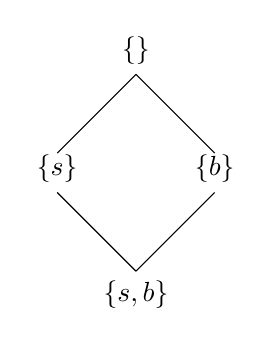
\begin{tikzpicture}
        \draw (0,5/2) -- (-1,3/2); 
        \draw (0,5/2) -- (1,3/2);
        \draw (-1,1) -- (0,0);
        \draw (1,1) -- (0,0);    

        \draw (0,5/2) node[above]{$\{\}$};
        \draw (-1,1) node[above]{$\{s\}$};
        \draw (1,1) node[above]{$\{b\}$};
        \draw (0,0) node[below]{$\{s,b\}$};
    \end{tikzpicture}
    \caption{Figure for generality ordering lattice for \{s,b\}}
    \label{fig:generality_ordering_lattice}
\end{figure}

\noindent
"Anti-monotonicity" principle: if $I_{1} \subseteq I_{2}$ (that is, $I_{1}$ is more general than $I_{2}$ then $freq(I_{1},D) \ge freq(I_{2},D)$, since it has more supersets) \\

\noindent
There are two borders: specific borders and general borders. 
\begin{enumerate}
    \item S-set = \{$I \subseteq \mathscr{I} | I$ satisfies min and max frequency thresholds, and there is no $J \subseteq \mathscr{I}$ that is strictly more specific than $I$ and also satisfies the thresholds\}. $\rightarrow$ meaning that \textbf{S is the most specific solution}, it contains all maximall solutions, solution that cannot be extended with extra items. 
    \item G-set = \{$I \subseteq \mathscr{I} | I$ satisfies min and max frequency thresholds, and there is no $J \subseteq \mathscr{I}$ that is strictly more geeneral than $I$\}. $\rightarrow$ meaning that \textbf{G is the most general solution}, it contains all minimal solutions, solution that cannot be deleted.
\end{enumerate}

\noindent
Concept-learning = 100\% frequency on the positives and 0\% frequency on the negatives.

\subsection{Enumeration Algorithms}
The naive algorithm for frequent itemset mining is shown as below: \\
\tabto{0mm} \textbf{Input:}
\tabto{5mm} a set of transactions $D$,
\tabto{5mm} a set of items $\mathscr{I}$,
\tabto{5mm} a frequency threshold $c$.
\tabto{0mm} Queue = \{\{\}\} \textcolor{cyan}{\emph{\% Empty set is also a itemset}}
\tabto{0mm} \textbf{for all} $I \in Queue$ \textbf{do}
\tabto{5mm} \textbf{if} $freq(I,D) \ge c$
\tabto{10mm} \textbf{then} output I
\tabto{10mm} add all $I \cup \{i\}$ to Queue (with $i \in \mathscr{I} - I$) \textcolor{cyan}{\emph{\% Add, s,c,b,m to \{\} to make \{s\}, \{c\}, \{b\}, \{m\}}}
\tabto{0mm} \textbf{end for}

\noindent
\\ Improvement: the naive algorithm has too many redundant examples, "lexicographic order" can be used to improve the efficiency. Symmetry breaking: impose the order $s > m > c > b$, and never add an element to a set $I$ if it smaller than the smallest element in the set. \emph{Every set is only generated once and we get a tree instead of a graph.} The algorithm is shown as below \textbf{(min + max + lexicographic)}:

\tabto{0mm} \textbf{Input:}
\tabto{5mm} a set of pos transactions \emph{Pos},
\tabto{5mm} a set of neg transactions \emph{Neg},
\tabto{5mm} a set of items $\mathscr{I}$,
\tabto{5mm} frequency thresholds $t_{1}, t_{2}$
\tabto{0mm} Queue = \{\{\}\}
\tabto{0mm} \textbf{for all} $I \in Queue$ \textbf{do}
\tabto{5mm} \textbf{if} $freq(I, Pos) > t_{1}$
\tabto{10mm} \textbf{then if} \textcolor{red}{$freq(I, Neg) \le t_{2}$} \textcolor{cyan}{\emph{\% This Neg can be Pos, too, but the truth meaning is $t^{\prime} \ge freq(I, Pos) \le t^{\prime \prime}$}}
\tabto{15mm} \textbf{then} output $I$
\tabto{20mm} add all $I \cup \{i\}$ to Queue (with $i \in \mathscr{I} - I$ and \textcolor{red}{$i$ lexicographically smaller than elements of $I$})
\tabto{0mm} \textbf{end for}

\subsection{Summary}
\begin{enumerate}
    \item The basic concept-learning - frequent itemsets mining
    \item min + max is just  ont type of constraints
    \item 100\% frequency on positives and 0\% on negatives = concept-learning with version spaces
    \item Frequent patterns can be turned in association rules to make predictions - similar to Naive Bayes (Probabilistic Machine Learning)
\end{enumerate}

\pagebreak
